\documentclass[11pt]{article}
\usepackage[margin=1in]{geometry}
\usepackage{xcolor}
\usepackage{amsmath,amssymb,amsthm,bm,booktabs,graphicx,hyperref,algorithm,algpseudocode}
\usepackage[capitalise]{cleveref}
\hypersetup{colorlinks=true,linkcolor=blue!50!black,citecolor=blue!50!black,urlcolor=blue!50!black}

\newcommand{\bb}{\bm\beta}
\newcommand{\bd}{\bm\delta}
\newcommand{\by}{\mathbf y}
\newcommand{\bX}{\mathbf X}
\newcommand{\bI}{\mathbf I}
\newcommand{\bV}{\mathbf V}
\newcommand{\bU}{\mathbf U}
\newcommand{\bQ}{\mathbf Q}
\newcommand{\bB}{\mathbf B}
\newcommand{\bA}{\mathbf A}
\newcommand{\bS}{\mathbf S}
\newcommand{\bvb}{\mathbf b}
\newcommand{\bmm}{\mathbf m}
\newcommand{\N}{\mathcal N}
\newcommand{\tr}{\operatorname{tr}}
\newcommand{\diag}{\operatorname{diag}}

\IfFileExists{timing.tex}{\newcommand{\tmeta}{22.6}
\newcommand{\tbrr}{2.5}
}{\newcommand{\tmeta}{?}\newcommand{\tbrr}{?}}

\title{metaBRR: random-effects meta-analytic Bayesian ridge regression\\
\large with an exact, \texttt{BayesianRidge}-speed fitting algorithm}
\author{}
\date{\today}

\begin{document}
\maketitle

\begin{abstract}
Bayesian ridge regression (BRR) with evidence-maximised hyperparameters is a strong,
tuning-free baseline for polygenic prediction. When individual-level data come from
several cohorts, pooled BRR assumes a single effect vector, while per-cohort BRR wastes
sample size. We describe metaBRR, which gives every cohort its own coefficient vector
$\bb_k$, drawn from a learned Gaussian random-effects prior centred on a shared vector
$\bb_0$. All three variance hyperparameters are learned by type-II maximum likelihood.
The key computational observation is that, for a fixed heterogeneity ratio
$r=\alpha/\lambda_\delta$, integrating out the cohort deviations reduces metaBRR
\emph{exactly} to an ordinary BRR on whitened data. Hence scikit-learn's spectral MacKay
updates can be reused unchanged inside a one-dimensional search over $r$. In simulations
with $N=10{,}000$ individuals in 12 cohorts and $P=2{,}000$ variants, metaBRR matches
pooled BRR when effects are homogeneous. It increasingly outperforms both pooled and
per-cohort BRR as cross-cohort heterogeneity grows, and it accurately recovers the
cross-cohort genetic correlation.
\end{abstract}

\section{Model}
We observe cohorts $k=1,\dots,K$ with genotypes $\bX_k\in\mathbb R^{n_k\times P}$ and
phenotypes $\by_k\in\mathbb R^{n_k}$, $N=\sum_k n_k$. Each cohort has its own intercept,
handled by centring $\bX_k$ and $\by_k$ within cohort. The model is
\begin{align}
\by_k \mid \bb_k &\sim \N(\bX_k\bb_k,\ \alpha^{-1}\bI_{n_k}), \\
\bb_k &= \bb_0 + \bd_k, \qquad \bd_k \sim \N(\mathbf 0,\ \lambda_\delta^{-1}\bI_P), \\
\bb_0 &\sim \N(\mathbf 0,\ \lambda_0^{-1}\bI_P).
\end{align}
Marginally, $\operatorname{Var}(\beta_{kj})=\lambda_0^{-1}+\lambda_\delta^{-1}$ and
$\operatorname{Cov}(\beta_{kj},\beta_{lj})=\lambda_0^{-1}$ for $k\neq l$. The
cross-cohort correlation of a variant's effect, the analogue of a trans-cohort genetic
correlation, is
\begin{equation}
\rho = \frac{\lambda_0^{-1}}{\lambda_0^{-1}+\lambda_\delta^{-1}}.
\end{equation}
$\rho=1$ ($\lambda_\delta\to\infty$) recovers pooled BRR. $\rho\to 0$ with
$\lambda_0^{-1}+\lambda_\delta^{-1}$ fixed gives independent per-cohort BRRs that share
their prior variance and noise precision. As in scikit-learn's \texttt{BayesianRidge},
$\alpha$ and $\lambda_0$ get weak $\mathrm{Gamma}(10^{-6},10^{-6})$ hyperpriors, and
hyperparameters are set by maximising the (penalised) marginal likelihood.

\section{Exact reduction to Bayesian ridge}
\paragraph{Integrating out the deviations.} Define the heterogeneity ratio
$r=\alpha/\lambda_\delta = \tau_\delta^2/\sigma^2$, the per-variant heterogeneity variance
in units of the noise variance. Integrating out $\bd_k$ gives
\begin{equation}
\by_k\mid\bb_0 \sim \N\!\big(\bX_k\bb_0,\ \alpha^{-1}(\bI+r\bX_k\bX_k^\top)\big),
\qquad k=1,\dots,K \text{ independent given }\bb_0.
\end{equation}
Let $\mathbf W_k=(\bI+r\bX_k\bX_k^\top)^{-1/2}$, $\tilde\by_k=\mathbf W_k\by_k$ and
$\tilde\bX_k=\mathbf W_k\bX_k$. Then $\tilde\by_k\mid\bb_0\sim\N(\tilde\bX_k\bb_0,\alpha^{-1}\bI)$
with $\bb_0\sim\N(0,\lambda_0^{-1}\bI)$, which is \emph{exactly} Bayesian ridge regression
in $(\alpha,\lambda_0)$ on the stacked whitened data. The change of variables
contributes a Jacobian, so
\begin{equation}\label{eq:ev}
\log p(\by\mid\alpha,\lambda_0,r) = \log p_{\mathrm{BRR}}(\tilde\by\mid\tilde\bX;\alpha,\lambda_0)
\;-\;\tfrac12\sum_k\log\det(\bI+r\bX_k\bX_k^\top).
\end{equation}

\paragraph{Spectral form.} Compute once the thin SVD
$\bX_k=\bU_k\bS_k\bV_k^\top$ with $\bS_k=\diag(\mathbf s_k)$ of rank $q_k\le\min(n_k,P)$.
Also compute the rotated phenotypes $\mathbf z_k=\bU_k^\top\by_k$ and the residual norm
$e_k=\|\by_k\|^2-\|\mathbf z_k\|^2$. Every whitened quantity is then diagonal in the
per-cohort singular bases. Writing $d_{kj}(r)=1/(1+rs_{kj}^2)$:
\begin{align}
\bB(r) &:= \textstyle\sum_k\tilde\bX_k^\top\tilde\bX_k = \sum_k \bV_k\diag(s_{kj}^2d_{kj})\bV_k^\top, \\
\bvb(r) &:= \textstyle\sum_k\tilde\bX_k^\top\tilde\by_k = \sum_k \bV_k\big(s_{kj}d_{kj}z_{kj}\big)_j,\\
\|\tilde\by\|^2 &= \textstyle\sum_k\big(\sum_j d_{kj}z_{kj}^2 + e_k\big), \qquad
\log\det(\bI+r\bX_k\bX_k^\top) = -\textstyle\sum_j\log d_{kj}.
\end{align}

\paragraph{Inner loop: BayesianRidge in the eigenbasis of $\bB(r)$.} For each $r$ we
eigendecompose $\bB(r)=\bQ\bm\Lambda\bQ^\top$ once and set $\mathbf c=\bQ^\top\bvb$. With
$\bm\Lambda$ fixed, every quantity in scikit-learn's MacKay loop costs $O(P)$:
\begin{align}
\hat{\bmm} &= \mathbf c\oslash(\bm\Lambda+\lambda_0/\alpha), &
\mathrm{SSE} &= \|\tilde\by\|^2-2\hat\bmm^\top\mathbf c+\hat\bmm^\top\bm\Lambda\hat\bmm, &
\gamma &= \textstyle\sum_j \frac{\alpha\Lambda_j}{\lambda_0+\alpha\Lambda_j},\\
\lambda_0 &\leftarrow \frac{\gamma+2\lambda_1}{\|\hat\bmm\|^2+2\lambda_2}, &
\alpha &\leftarrow \frac{N-\gamma+2\alpha_1}{\mathrm{SSE}+2\alpha_2}. &&
\end{align}
These updates are identical to \texttt{BayesianRidge}. At convergence the profile
evidence~\eqref{eq:ev} is
\begin{equation}
\mathcal L(r)=\tfrac12\Big[P\log\lambda_0+N\log\alpha-\alpha\,\mathrm{SSE}-\lambda_0\|\hat\bmm\|^2
-\textstyle\sum_j\log(\lambda_0+\alpha\Lambda_j)-N\log2\pi\Big]
+\tfrac12\textstyle\sum_{k,j}\log d_{kj}
\end{equation}
plus the Gamma hyperprior terms.

\paragraph{Outer loop over $r$.} $\mathcal L(r)$ is maximised over $\log r$. We
evaluate it on a coarse log-spaced grid of 9 points spanning $[10^{-4},10^4]/\bar s^2$,
where $\bar s^2$ is the mean squared singular value. We then refine with bounded Brent
search between the neighbours of the best grid point. Finally we compare against the
homogeneous limit $r=0$, which is pooled BRR exactly. Each evaluation costs one $P\times P$ Gram accumulation and one symmetric eigendecomposition.

\paragraph{Cohort-specific posterior means.} The joint posterior is Gaussian, and
$\mathbb E[\bd_k\mid\bb_0,\by]$ is linear in $\bb_0$. Hence
$\mathbb E[\bb_k\mid\by]=\hat\bb_0+\mathbb E[\bd_k\mid\bb_0=\hat\bb_0,\by]$, with
$\hat\bb_0=\bQ\hat\bmm$, and
\begin{equation}
\hat\bb_k = \hat\bb_0 + (\lambda_\delta\bI+\alpha\bX_k^\top\bX_k)^{-1}\alpha\bX_k^\top(\by_k-\bX_k\hat\bb_0)
= \hat\bb_0 + \bV_k\Big(\frac{r s_{kj}}{1+rs_{kj}^2}\big(z_{kj}-s_{kj}\,\mathbf v_{kj}^\top\hat\bb_0\big)\Big)_j .
\end{equation}
Each cohort's estimate is the shared estimate plus a ridge fit of the cohort's residuals,
shrunk per singular direction by $rs^2/(1+rs^2)$. Directions that are well measured in
cohort $k$ ($rs^2\gg1$) follow that cohort's own data; poorly measured directions fall
back on $\hat\bb_0$. A new, unseen cohort is predicted with $\hat\bb_0$.

\paragraph{Complexity.} Preprocessing is one thin SVD per cohort,
$O(\sum_k n_kPq_k)$. Each outer evaluation costs $O(P^2\sum_kq_k+P^3)$, and the inner
MacKay iterations are $O(P)$ each. A naive implementation would instead work with the
$(K+1)P$-dimensional joint posterior, at $O(K^3P^3)$ per hyperparameter update. With
$N=10^4$, $P=2{,}000$ and $K=12$, a full metaBRR fit including the $\approx$20 evidence
evaluations of the $r$ search takes a median of \tmeta\,s on a 12-core CPU, versus
\tbrr\,s for scikit-learn's pooled \texttt{BayesianRidge}.

\begin{algorithm}[t]
\caption{metaBRR}\label{alg}
\begin{algorithmic}[1]
\State centre $\bX_k,\by_k$ within cohort; thin SVD $\bX_k=\bU_k\bS_k\bV_k^\top$; $\mathbf z_k\gets\bU_k^\top\by_k$
\Function{Profile}{$r$}
  \State form $\bB(r)$, $\bvb(r)$, $\|\tilde\by\|^2$; eigendecompose $\bB=\bQ\bm\Lambda\bQ^\top$; $\mathbf c\gets\bQ^\top\bvb$
  \State run \texttt{BayesianRidge} MacKay updates for $(\alpha,\lambda_0)$ in spectral form until convergence
  \State \Return $\mathcal L(r)$, $\alpha$, $\lambda_0$, $\hat\bb_0=\bQ\hat\bmm$
\EndFunction
\State $r^\star\gets\arg\max_r\mathcal L(r)$ (log grid + Brent; compare with $r=0$)
\State $\lambda_\delta\gets\alpha/r^\star$; $\hat\bb_k\gets\hat\bb_0+\bV_k\,\diag\!\big(\tfrac{rs}{1+rs^2}\big)(\mathbf z_k-\bS_k\bV_k^\top\hat\bb_0)$
\end{algorithmic}
\end{algorithm}

\paragraph{Verification.} The unit tests (\texttt{tests/test\_metabrr.py}) check three
things. (i) The spectral evidence and the posterior means of $\bb_0$ and every $\bb_k$
agree with a dense computation, both the explicit $N\times N$ marginal covariance and
the $(K+1)P$-dimensional joint posterior, for $n_k<P$ and $n_k>P$. (ii) The learned
$(\alpha,\lambda_0,\lambda_\delta)$ are a local maximum of the dense evidence. (iii) At
$r=0$ the fit reproduces scikit-learn's \texttt{BayesianRidge} exactly.

\section{Simulation}
\paragraph{Design.} $K=12$ cohorts of $n_k=833$ training individuals ($N\approx10^4$)
and 500 held-out test individuals each, with $P=2{,}000$ variants. Ancestral allele
frequencies are drawn from $U(0.05,0.5)$. Cohort frequencies follow a Balding--Nichols
model with $F_{ST}=0.02$, and genotypes are standardised within cohort. Effects are
$\bb_k=\sqrt\rho\,\mathbf b_0+\sqrt{1-\rho}\,\mathbf d_k$ with
$\mathbf b_0,\mathbf d_k\sim\N(0,\tfrac{h^2}{P}\bI)$, so every cohort has SNP-heritability
$h^2$ and cross-cohort genetic correlation $\rho$. Noise variance is $1-h^2$, and each
cohort gets a random mean shift. We vary $h^2\in\{0.1,0.25,0.5,0.75\}$ and heterogeneity
$1-\rho\in\{0,0.1,0.25,0.5,0.75,1\}$, with 3 replicates per setting.

\paragraph{Methods.} (1) \emph{BRR (pooled)}: \texttt{BayesianRidge} on the pooled,
cohort-centred data. (2) \emph{BRR (per cohort)}: a separate \texttt{BayesianRidge} per
cohort. (3) \emph{metaBRR}: cohort-specific $\hat\bb_k$. (4) \emph{metaBRR (shared
$\beta_0$)}: metaBRR's $\hat\bb_0$ applied to every cohort, i.e.\ the prediction for a
new cohort. Accuracy is the within-cohort test $R^2_g$, the squared correlation between
predicted and true genetic value, averaged over cohorts. Phenotype $R^2$ is in
\cref{fig:r2y}.

\paragraph{Results.} \Cref{fig:r2g,tab:r2g} show prediction accuracy.
\begin{itemize}
\item \emph{No heterogeneity ($\rho=1$).} metaBRR learns $\hat\rho\approx1$ (mean
$0.96$) and matches pooled BRR to within $0.006$ $R^2_g$ in every replicate. The extra
random effect therefore costs essentially nothing when it is not needed.
\item \emph{Increasing heterogeneity.} The advantage of metaBRR over pooled BRR grows
monotonically with $1-\rho$ and with $h^2$ (\cref{fig:gain}). Averaged over $h^2$, the
$R^2_g$ gain is $0.015$, $0.050$, $0.090$ and $0.138$ at $\rho=0.75$, $0.5$, $0.25$ and
$0$. At $h^2=0.75$ and $\rho=0.25$, metaBRR attains $R^2_g=0.365$, against $0.186$ for
pooled and $0.282$ for per-cohort BRR. At intermediate $\rho$ metaBRR beats \emph{both}
baselines: it borrows strength across cohorts for the shared component while still
fitting cohort-specific deviations.
\item \emph{No sharing ($\rho=0$).} Pooled BRR collapses to $R^2_g\approx0$, while
metaBRR learns $\hat\rho\approx0.02$ and matches per-cohort BRR exactly.
\item \emph{Heterogeneity estimation.} The estimated cross-cohort correlation $\hat\rho$
tracks the truth closely across all settings (\cref{fig:rho}). It is noisier at low
$h^2$, where there is little genetic signal to estimate it from.
\item \emph{Shared $\hat\bb_0$.} Used alone, metaBRR's $\hat\bb_0$ predicts about as
well as pooled BRR and slightly better under heterogeneity. It is the appropriate
predictor for an unseen cohort.
\end{itemize}

\begin{figure}[t]
\centering
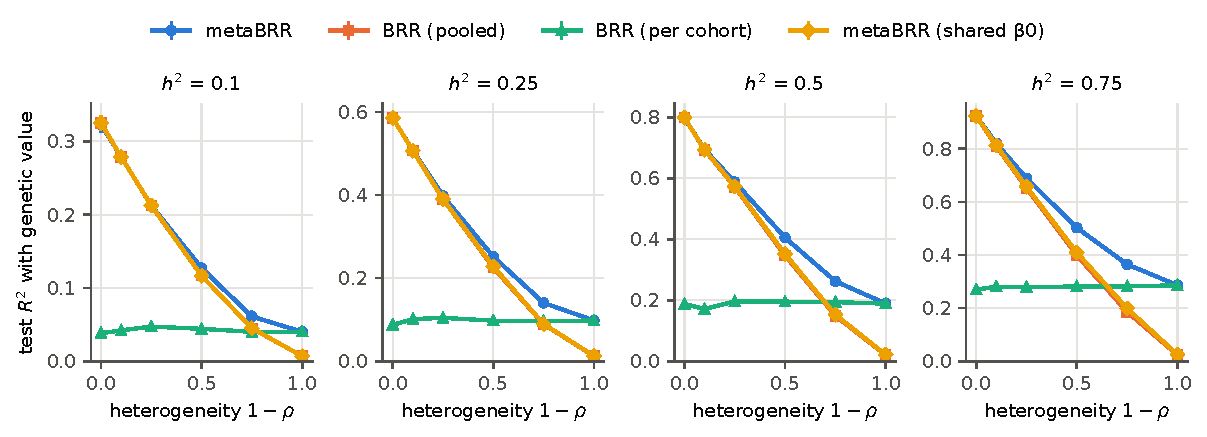
\includegraphics[width=\textwidth]{fig_r2g.pdf}
\caption{Test-set $R^2$ between predicted and true genetic value, averaged over cohorts
(mean $\pm$ s.e.\ over 3 replicates). $N=10^4$ in $K=12$ cohorts, $P=2{,}000$.}
\label{fig:r2g}
\end{figure}

\begin{figure}[t]
\centering
\begin{minipage}{0.48\textwidth}\centering
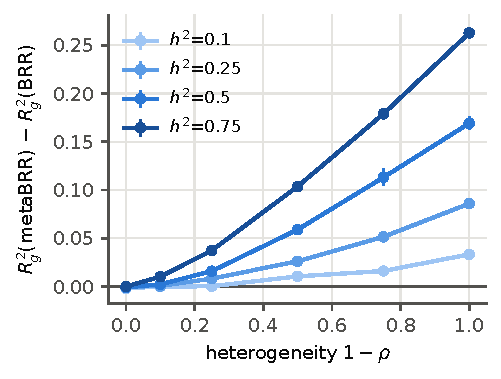
\includegraphics[width=\linewidth]{fig_gain.pdf}
\caption{Gain of metaBRR over pooled BRR in $R^2_g$.}\label{fig:gain}
\end{minipage}\hfill
\begin{minipage}{0.45\textwidth}\centering
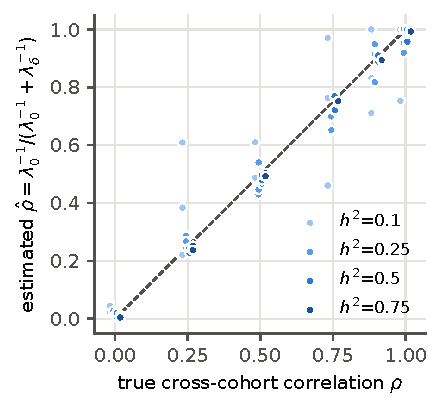
\includegraphics[width=\linewidth]{fig_rho.pdf}
\caption{Estimated vs.\ true cross-cohort correlation (each point one replicate).}\label{fig:rho}
\end{minipage}
\end{figure}

\begin{figure}[t]
\centering
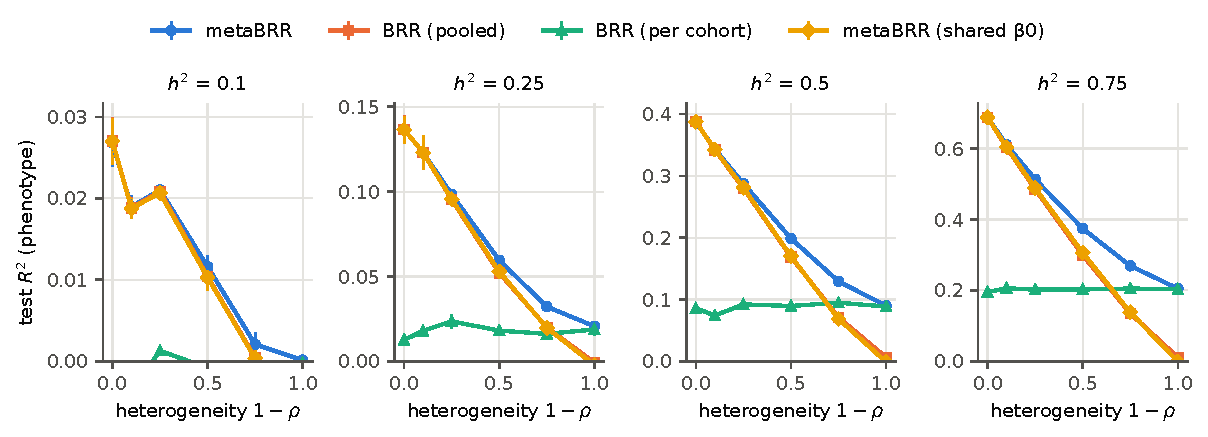
\includegraphics[width=\textwidth]{fig_r2y.pdf}
\caption{As \cref{fig:r2g}, but test-set phenotype $R^2$ (upper bound $h^2$).}
\label{fig:r2y}
\end{figure}

\begin{table}[t]
\centering\small
\caption{Mean test $R^2_g$ (best in bold).}\label{tab:r2g}
\begin{tabular}{rrcccc}
\toprule
$h^2$ & $\rho$ & BRR (pooled) & BRR (per cohort) & metaBRR (shared $\hat{\bm\beta}_0$) & metaBRR \\
\midrule
0.1 & 0 & 0.007 & \textbf{0.040} & 0.007 & 0.040 \\
0.1 & 0.25 & 0.045 & 0.040 & 0.045 & \textbf{0.061} \\
0.1 & 0.5 & 0.117 & 0.044 & 0.117 & \textbf{0.127} \\
0.1 & 0.75 & 0.212 & 0.047 & \textbf{0.213} & 0.212 \\
0.1 & 0.9 & 0.279 & 0.042 & \textbf{0.279} & 0.279 \\
0.1 & 1 & \textbf{0.325} & 0.038 & 0.325 & 0.323 \\
0.25 & 0 & 0.012 & 0.098 & 0.013 & \textbf{0.098} \\
0.25 & 0.25 & 0.089 & 0.097 & 0.090 & \textbf{0.140} \\
0.25 & 0.5 & 0.225 & 0.098 & 0.228 & \textbf{0.251} \\
0.25 & 0.75 & 0.390 & 0.104 & 0.390 & \textbf{0.398} \\
0.25 & 0.9 & 0.507 & 0.101 & 0.507 & \textbf{0.507} \\
0.25 & 1 & \textbf{0.585} & 0.088 & 0.585 & 0.585 \\
0.5 & 0 & 0.020 & 0.189 & 0.021 & \textbf{0.189} \\
0.5 & 0.25 & 0.149 & 0.194 & 0.153 & \textbf{0.262} \\
0.5 & 0.5 & 0.346 & 0.195 & 0.352 & \textbf{0.405} \\
0.5 & 0.75 & 0.572 & 0.196 & 0.573 & \textbf{0.587} \\
0.5 & 0.9 & 0.692 & 0.171 & 0.693 & \textbf{0.695} \\
0.5 & 1 & \textbf{0.798} & 0.188 & 0.798 & 0.797 \\
0.75 & 0 & 0.024 & 0.286 & 0.026 & \textbf{0.286} \\
0.75 & 0.25 & 0.186 & 0.282 & 0.199 & \textbf{0.365} \\
0.75 & 0.5 & 0.399 & 0.282 & 0.410 & \textbf{0.503} \\
0.75 & 0.75 & 0.652 & 0.278 & 0.657 & \textbf{0.689} \\
0.75 & 0.9 & 0.810 & 0.281 & 0.812 & \textbf{0.820} \\
0.75 & 1 & 0.923 & 0.270 & \textbf{0.923} & 0.923 \\
\bottomrule
\end{tabular}

\end{table}


\section{Discussion and extensions}
metaBRR is a drop-in generalisation of BRR for multi-cohort individual-level data. It
costs one extra scalar search, and it nests pooled BRR ($r=0$). The reduction holds for
any $r$ shared across cohorts, which requires a common noise precision $\alpha$.
Cohort-specific $\alpha_k$ break the single-ratio structure, since each cohort would then
have its own $r_k=\alpha_k/\lambda_\delta$. A practical workaround is to rescale each
cohort's phenotype by an estimate of its residual SD first. Natural extensions are:
cohort-specific heterogeneity variances $\lambda_{\delta,k}$ (a $K$-dimensional outer
search, or EM); structured cohort covariance, e.g.\ by ancestry, with
$\operatorname{Cov}(\bb_k,\bb_l)=T_{kl}\bI$; and a summary-statistic version that
replaces $\bX_k^\top\bX_k$ with LD matrices.

\end{document}
